\section*{Question 5: Classification}

\subsection*{a)}
\begin{figure}[H]
\caption{Single layer perceptrons}
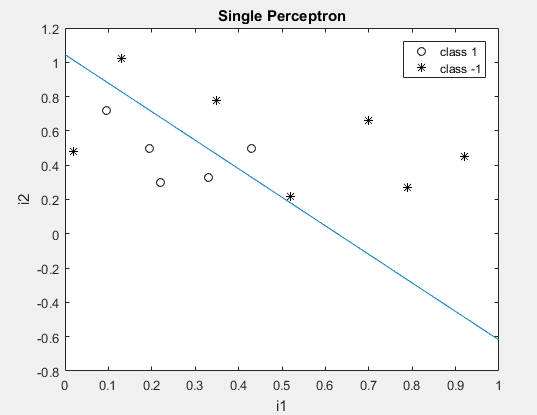
\includegraphics[width=8cm]{singlenonlin.png}
\centering
\end{figure}

Using the same code for the perceptron as in question 4, I was able to get a minimum of 2 classification errors. This means the data points are non-linearly separable. A multi-layer perceptron would be better in classifying this set of data.



\subsection*{b)}

\begin{figure}[H]
\caption{Multi layer perceptrons}
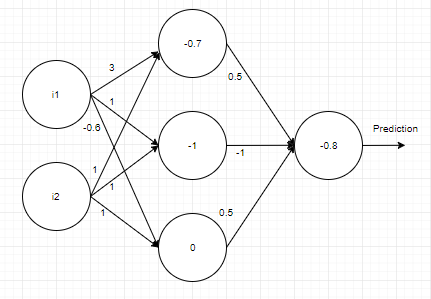
\includegraphics[width=8cm]{hidden.png}
\centering
\end{figure}

\begin{figure}[H]
\caption{Dividing lines of multi layer perceptron}
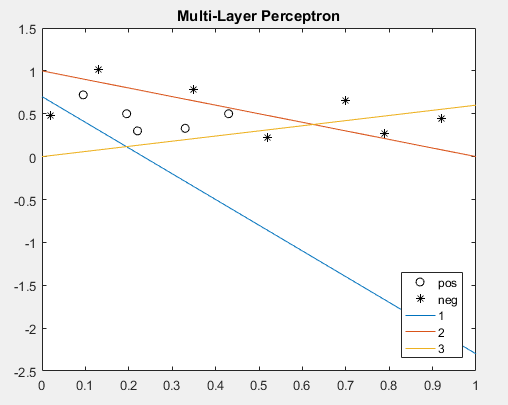
\includegraphics[width=8cm]{q5mlp.png}
\centering
\end{figure}

$w_{11} = 3, w_{12} = 1, w_{13} = -0.6$\\
$w_{21} = 1, w_{22} = 1, w_{23} = 1$\\
$b_1 = -0.7, b_2 = -1, b_3 = 0, b_4 = -0.8$\\